\documentclass[../main.tex]{subfiles}

\begin{document}

\subsection{Simulation and reinforcement learning}

% Describe detailed design and implementation of 
% the Proof of Concept (PoC) to prove the feasibility 
% of your design idea and deliver the core of your 
% project solution. It is highly recommended to design 
% and implement the core features of system by choosing 
% the most important/critical use cases (or important 
% component(s) from your high-level design) then design, 
% implement and test them.

% Design and implement part of your complete system. 
% It is expected that the PoC delivers 20% to 30% of 
% the important system use cases.

% Conduct initial PoC tests to demonstrate the 
% feasibility of the design idea of your solution. 
% This will help you refine your design and identify 
% potential technical and logistical issues that you 
% need to address to ensure your project success.

% Demonstrate your PoC to the examiners during the 
% senior project presentation.

The simulation and reinforcement learning are critical
components to achieve objective \ref{obj:drl}.
This part of the project starts with receiving
information about the targets' count, distribution
and mobility pattern
and ends with producing a file containing the weights
for the \gls{drl} model.
In our work described below, we have assumed certain
information about the targets but that shall change
with clients and types of the target visitation.

We have represented the targets in the simulation
as green 3D flat boxes
% as transparent 3D flat boxes
% with their \textsc{id}'s displayed on the top face
as can be seen in \cref{fig:one-target}. 
The basic shape and the colour green green were created by 
% The basic shape and transparency was created by 
defining a model 
in the \gls{sdf}
including its visual, collision and inertial properties.
Using the \textit{libgazebo7} development package, 
we have written a Gazebo plugin 
in c++ to describe custom properties and  
behaviour of the model.
Developing a Gazebo plugin is not a straightforward
process in our case, as explained later, due to 
the incompatibility between the Sphinx plugins and
our \textsc{os}.
% The main property is the model's \textsc{id} and 
% its placement
% while the main type of behaviour is its mobility pattern, 
Nevertheless, we have managed to program the targets' main type of behaviour which is its mobility pattern.
For the proof of concept, 
it has been set to be a straight line movement.
The \texttt{population} tag in \gls{sdf} was used 
to place the required number of targets (in this case 20)
following the assumed uniform probability distribution 
function supplied by the
client as shown in \cref{fig:target-population}.

\begin{figure}[tb]%
    \centering
    \subfloat[one target]{
    {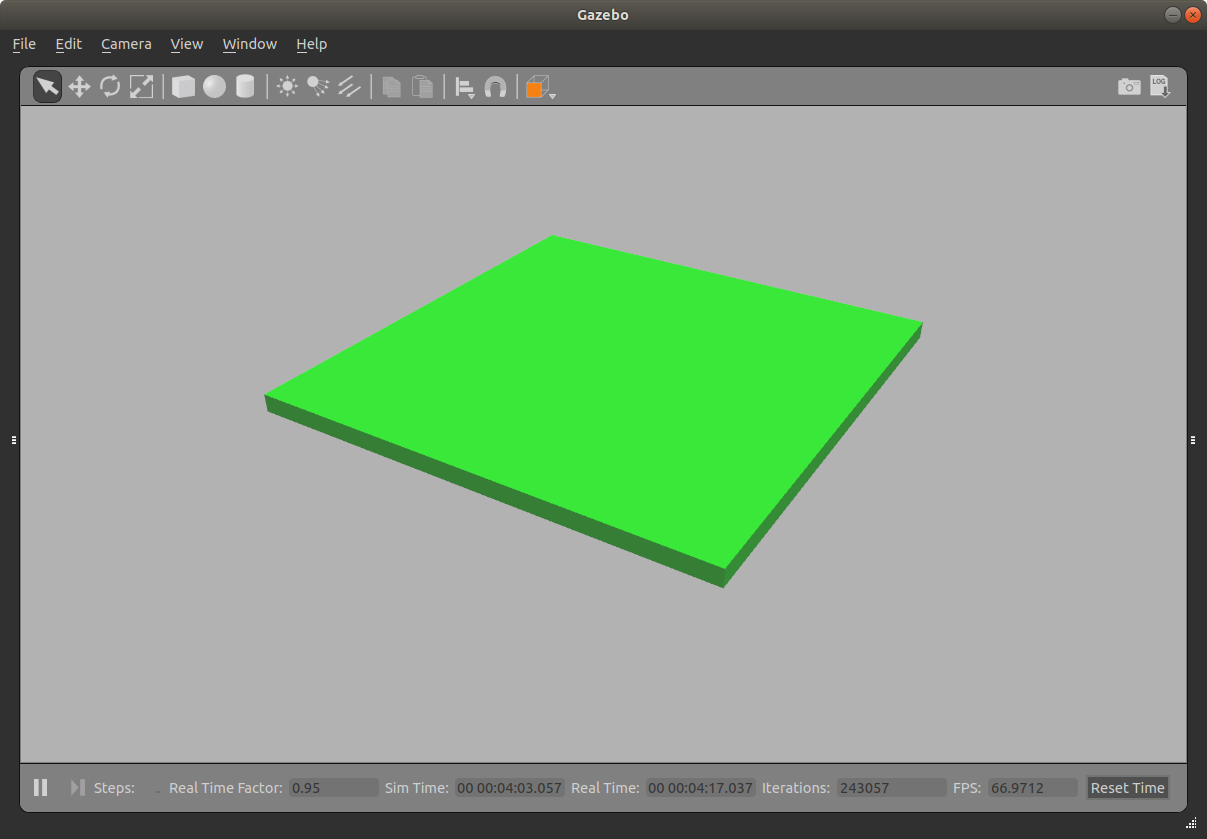
\includegraphics[width=7cm]{one-target} }
    \label{fig:one-target} }%
    \hspace{0.5cm}
    \subfloat[a population of targets]{
    {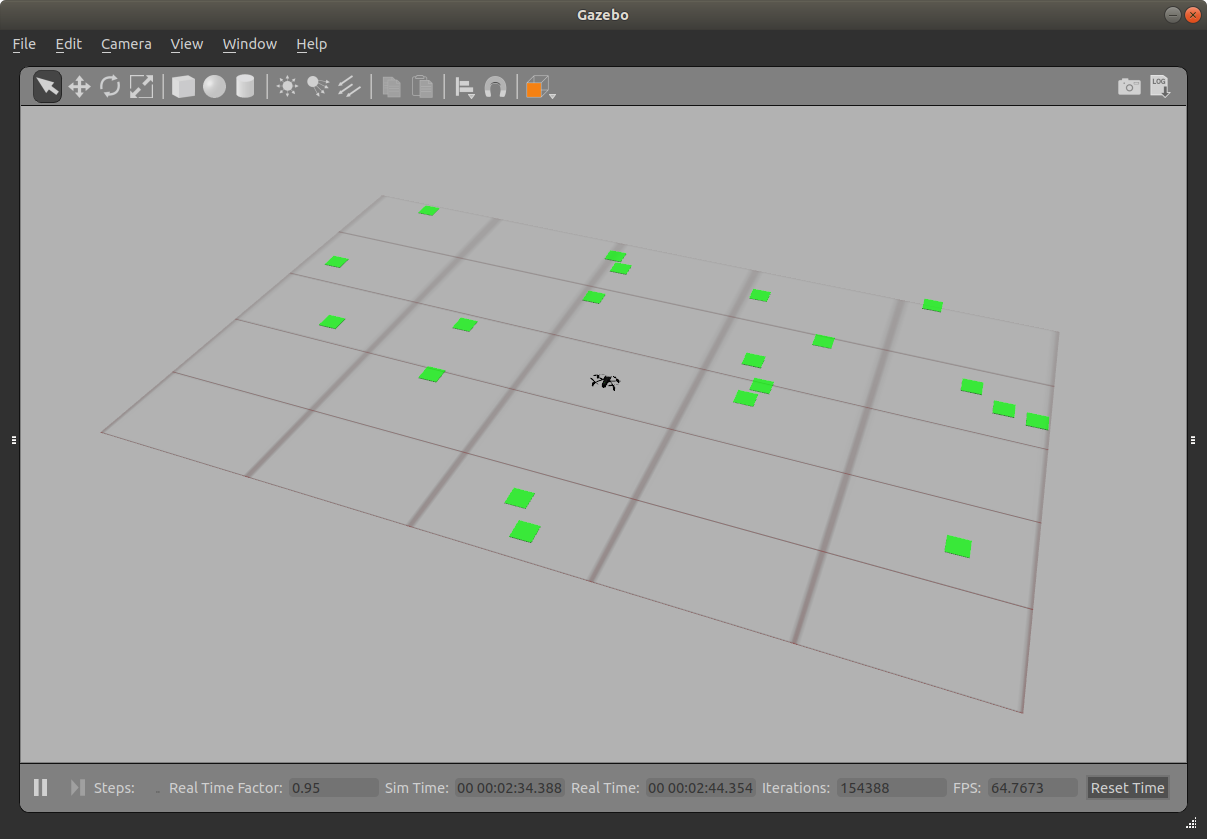
\includegraphics[width=7cm]{population} }
    \label{fig:target-population} }%
    \caption{%
        \protect\subref{fig:one-target} 
        A target represented as a model in Sphinx and
        \protect\subref{fig:target-population} 
        the target models are scattered across
        the ground following a set distribution.}%
    \label{fig:target}%
\end{figure}

% \caption{A target with its \textsc{id} on the
%     top represented as a model in Sphinx.}

The 3D model, properties and behaviour
of the \anafi drone is provided by Parrot in the 
form of a firmware. 
Both the drone's and the target's models were spawn
in Sphinx using the \gls{sdf} language.
With Sphinx running, the simulated \anafi drone 
started using
a virtual ethernet interface 
(with an \textsc{ip} of 10.202.0.1 by default) 
on the host computer.

Sphinx publishes data about the simulated drone,
one of which is its pose relative to
the world's origin that we have set to be the same
as the drone's take-off point. 
To read this positional data from a Python script, we 
subscribed to the Gazebo topic 
\texttt{/gazebo\-/default\-/pose\-/info}
in a separate thread so that the control signals
will not be blocked while reading the drone's positions.
In addition to receiving data from Sphinx, we have 
sent data to it using the \textsc{json-rpc} standard
with an instruction to disable
the simulation of the \anafi drone's battery
for the \gls{rl}'s purposes. This is important because
if the battery is simulated, the drone will 
perform badly while running
out of battery and after around 20 minutes, 
the drone will stop working and the whole system
needs to be re-spawn. For this reason, the drone's
battery was not simulated.

As for sending movement commands to the drone,
the Parrot Olympe was used.
In an \textsc{ide}, the Olympe library was imported
in a Python script. The library allowed us to connect
to the simulated drone by specifying the drone's
\textsc{ip}. Once the connection was established, 
we could send the Olympe control commands to the drone
to execute the visitation task. Which command to use
depends on the reinforcement learning.

The reinforcement learning was aided 
by another library called \gym.
We used it to facilitate developing the
\gls{drl} algorithm we are implementing and to 
teach the drone how to achieve the 
target visitation mission.
Specifically, \gym provides an abstract class 
called \texttt{Env}
which we have inherited and overridden the 
required unimplemented methods.
The action space is defined in the subclass, and its
elements call the necessary Olympe functions. 
The space consists of 9 movements: 
forward, backward, left,
right, forward-left, forward-right, backward-left,
backward-right and no-operation.
Similarly, the state space is composed of the 25 cells
making up the grid on the ground. 
The relationship and interaction between \gym, Olympe
and Sphinx are shown in \cref{fig:sim-flowchart}.

\begin{figure}[p]
    \centering
    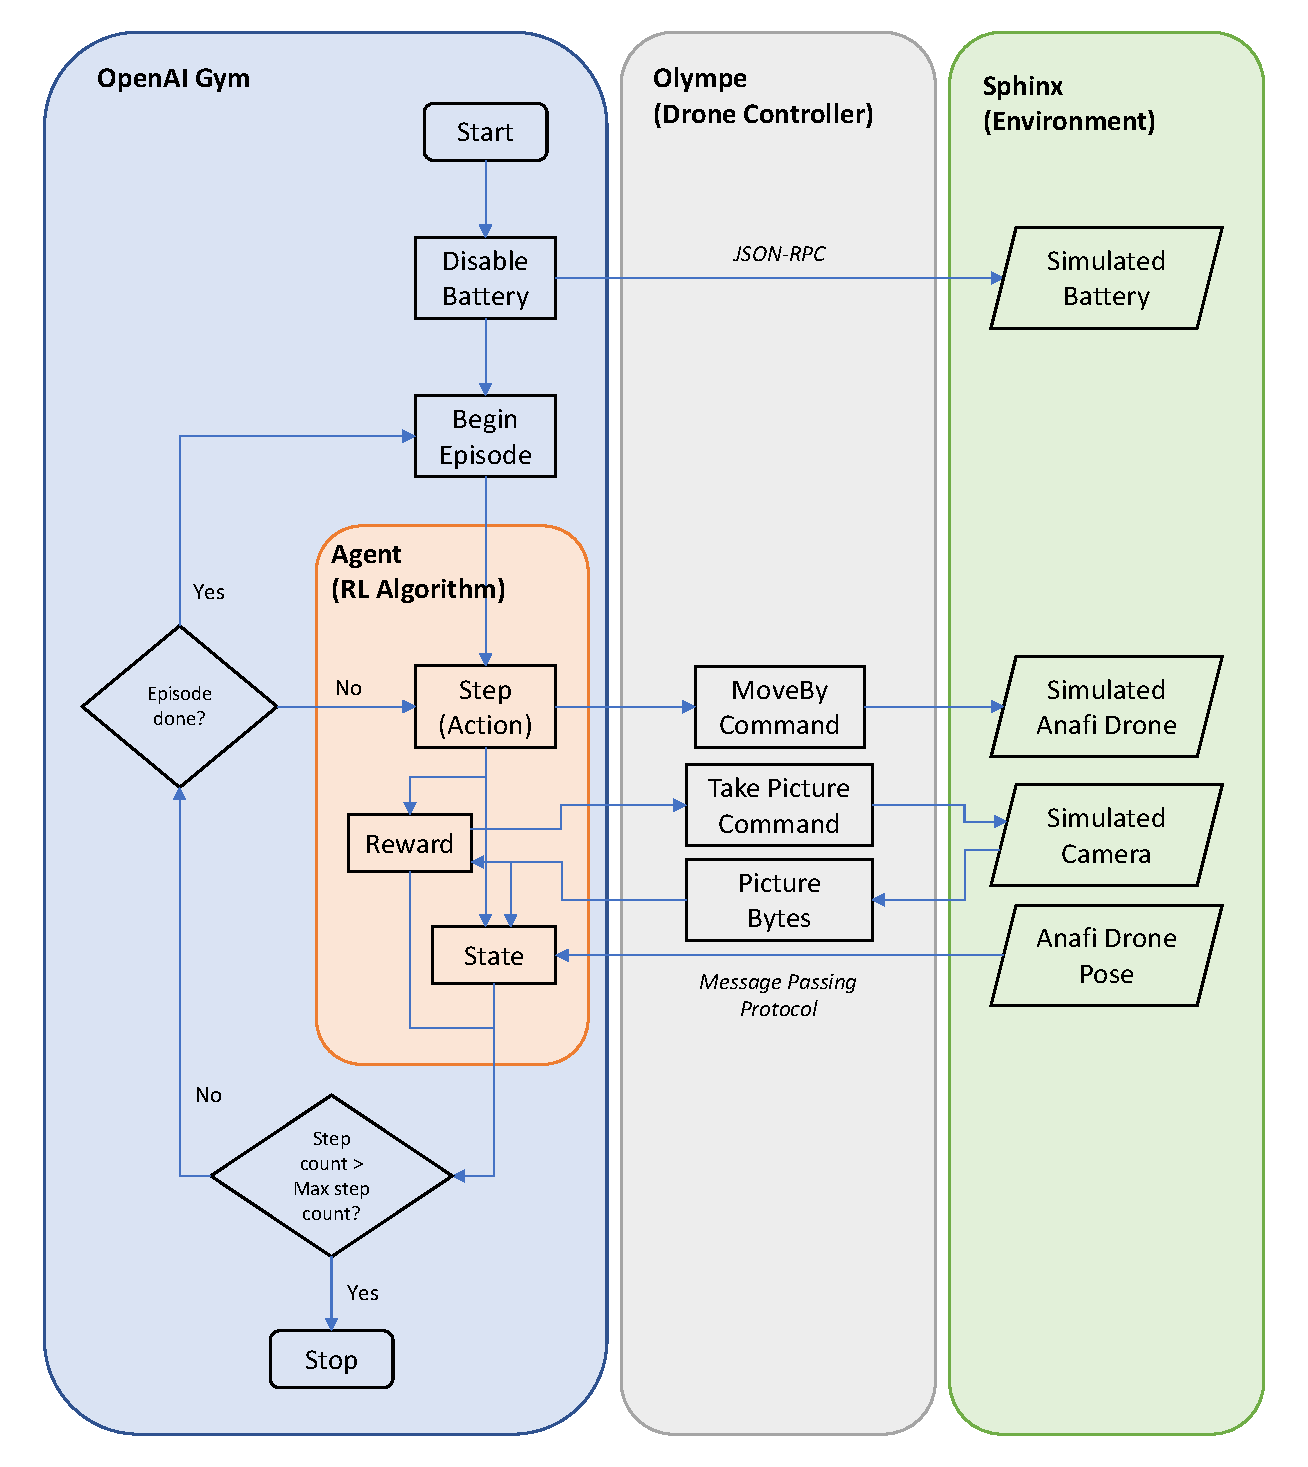
\includegraphics[width=1.0\textwidth]{sim-flowchart}
    \caption{A flowchart showing the training process
        of the reinforcement learning in the project
        and the interactions between the libraries
        and programs.}
    \label{fig:sim-flowchart}
\end{figure}

A crucial element of any \gls{rl} model
is the reward function. In this project, it
is the number of new targets that the drone has captured
in the cell that it has moved to. We have made the drone
to take a picture of the cell underneath it after 
every move and we have used object detection to
identify the targets and count their quantity. 
% checking if their \id's are not listed 
% in the already captured targets. 
In addition to object detection which is explained
in the succeeding \cref{sec:obj-detection}, developing this
aspect of the simulation involved 
setting the camera and position of the drone to ensure
the rewards are valid and accurate.

\Cref{fig:fov} shows the view from the drone's
simulated camera. The altitude was set such that
the \gls{fov} covers more than the cell underneath
but not more than half of the adjacent cells.
The reason for the larger coverage is that
the \anafi drone only uses a regular \gls{gps}.
This means that its coordinates are accurate only
to \SIrange{3}{5}{\meter}, but moving to another
cell involves
movements of less than \SI{2}{\meter}.
To minimise the errors and ensure that the current
cell will always be in the \gls{fov} even if the
movement is off by few centimeters, we made the camera
cover an area bigger than a cell. 
This however results in a more difficult
object detection because in addition to their 
\id's, we need to also distinguish between
the targets that are within the cell and 
those outside of it.
Another related question that has arisen is if we 
should consider the target that falls on the border 
as a reward such as that in \cref{fig:cell-one}. 
We have decided that we would do so if
the majority part of the target is inside the current
cell, although we realised that this will make the
object detection much harder.

\begin{figure}[tb]%
    \centering
    \subfloat[zero rewards]{
    {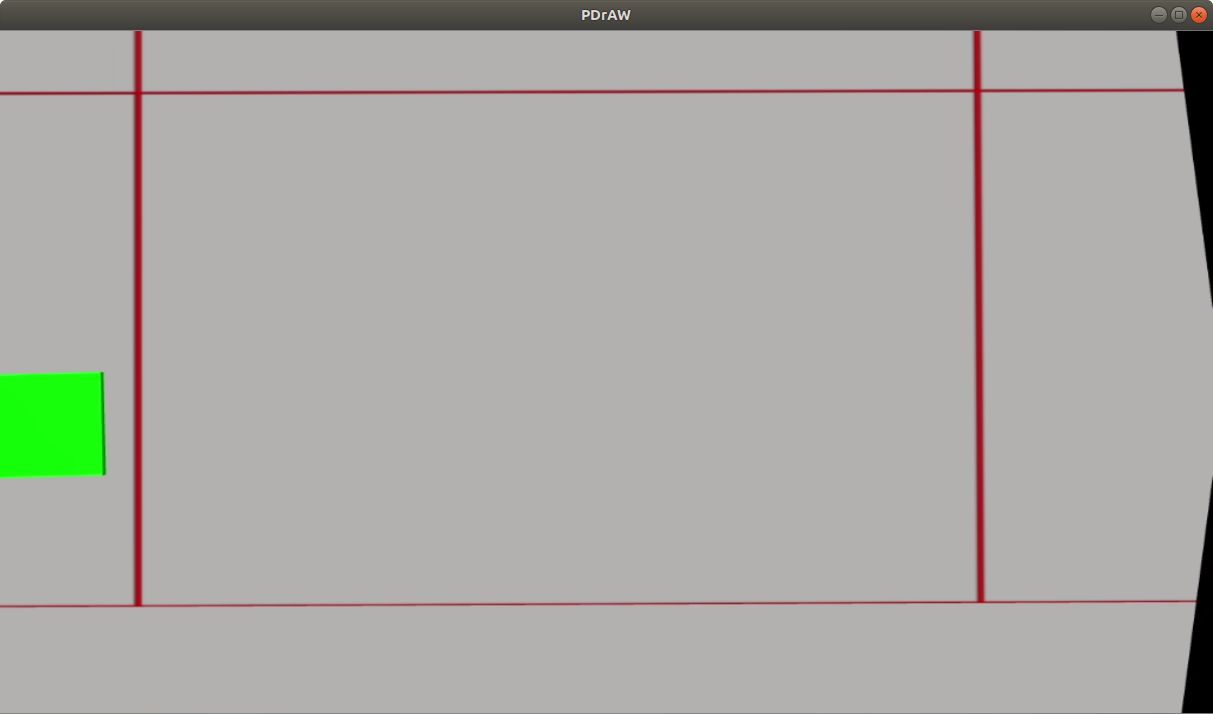
\includegraphics[width=4.5cm]{cell-empty} }
    \label{fig:cell-empty} }%
    \hspace{0.2cm}
    \subfloat[one reward]{
    {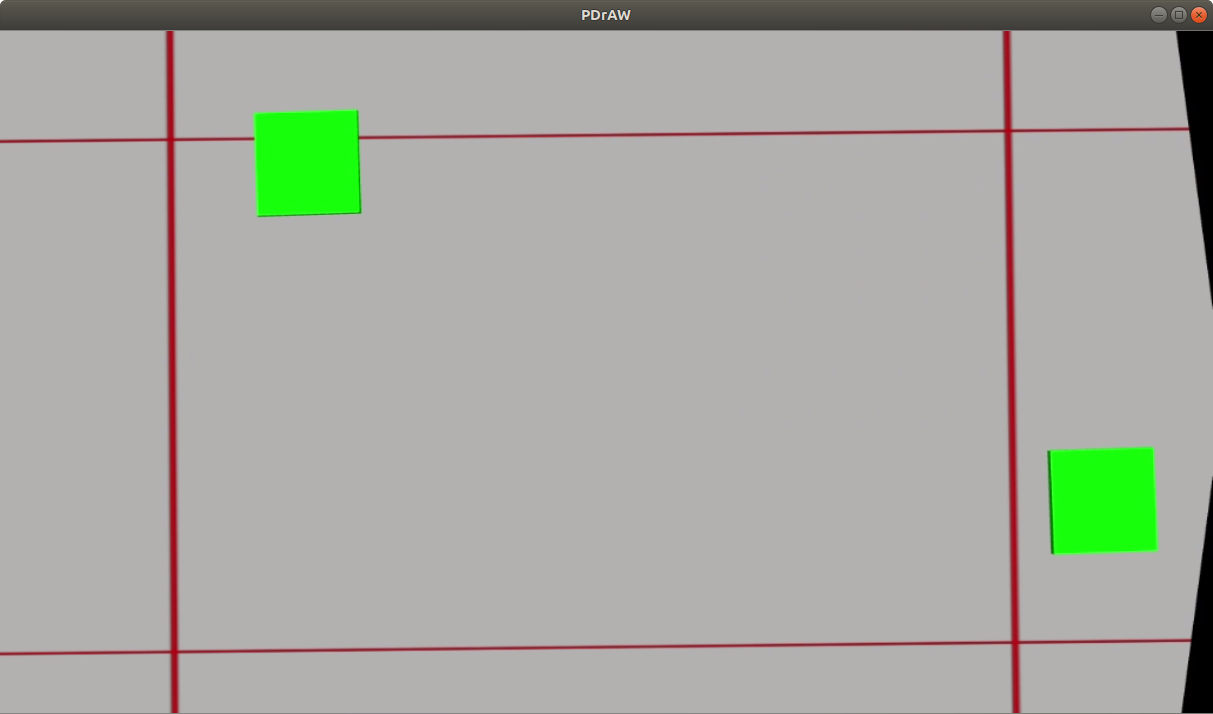
\includegraphics[width=4.5cm]{cell-one} }
    \label{fig:cell-one} }%
    \hspace{0.2cm}
    \subfloat[two rewards]{
    {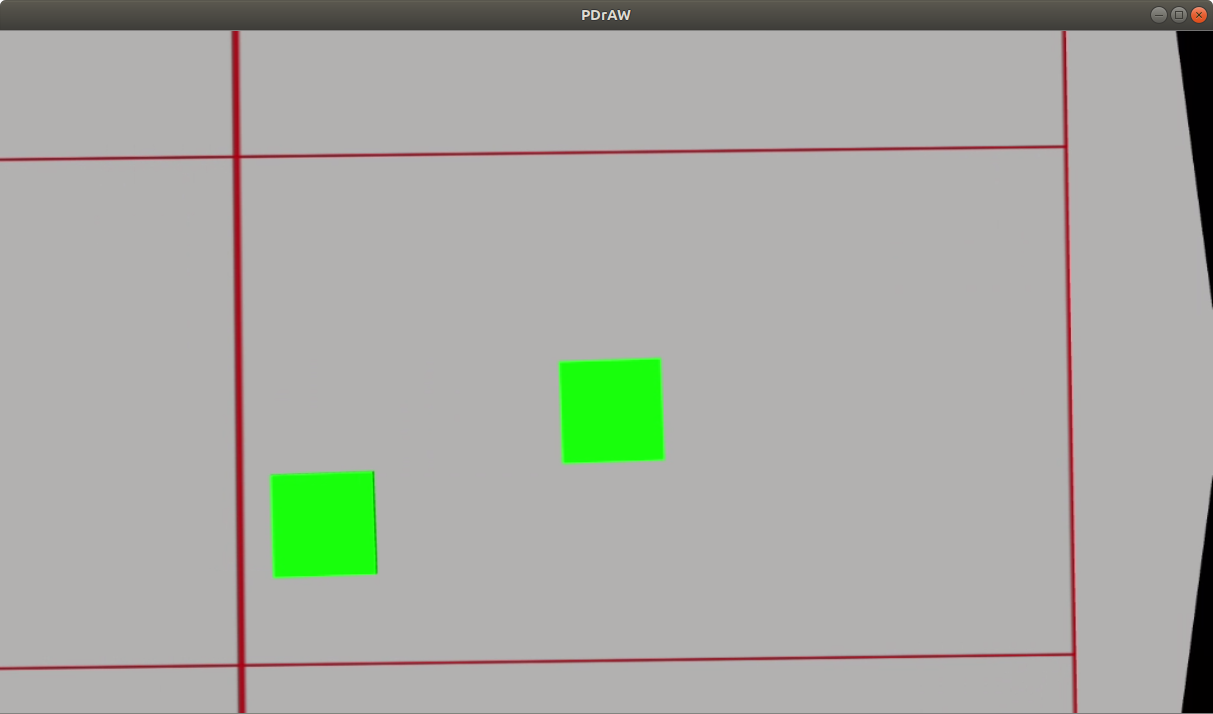
\includegraphics[width=4.5cm]{cell-two} }
    \label{fig:cell-two} }%
    \caption{%
        \protect The \gls{fov} of the \anafi drone
        during the training in the simulation
        showing multiple scenarios that the drone
        may encounter at each cell.}%
    \label{fig:fov}%
\end{figure}

A critical problem we have been facing 
is how to distinguish
between the targets. This is a required task in the
project's \gls{rl} training since 
the \gls{drl} model's state
includes the information about whether or not
the targets forming the reward have been seen 
during the current episode or not. 
At first, we came up with the idea of distinguishing them
with colours. However, it is not scalable 
as the 13\textsuperscript{th}
target and above will have to use 
one of the already taken colours
except with different shades. The bigger the number of
targets in the training, the harder it is to
distinguish between them in the object detection part
thus causing errors and inaccuracy. Hence, we decided
to use numbers by displaying a unique \id
to differentiate them, but
Sphinx does not provide that option by default.
A way to get around this is to develop a Gazebo plugin,
but this needs to be done using the \textit{libgazebo7} running
on Ubuntu 16.04 as opposed to Ubuntu 18.04 which we 
have chosen to use because the former 
is no longer supported.
We further solved this problem by using the Ubuntu 16.04
Docker container to write the plugin. While we managed
to successfully made the plugin, it unfortunately still
could not be used on our machine because \textit{libgazebo7}
uses some shared libraries whose versions can be only 
be run on Ubuntu 16.04. One such culprit is the 
\textit{libprotobuf.so.9} from the Google Protocol Buffer 
(Protobuf) used heavily by Sphinx but cannot be compiled
in Ubuntu 18.04. Consequently, 
to solve the problem of making each target distinct, 
we have decided that we would wait for the new
version of Sphinx running on the latest Gazebo
which Parrot will release soon. In case that does
not happen,
we will resort to installing Ubuntu 16.04 and develop
all of our project's simulation using it.

We have also done a preliminary test to see if
we could use an \gls{rl} algorithm
to teach the \anafi drone to fly to a certain
point in space. We used the Trust Region Policy
Optimization (\textsc{trpo}) from the Stable
Baselines3 (\textsc{sb}3) with similar action
and state spaces as the target visitation environment
setup described above.
After \SI{10000}{steps} and \SI{2}{hours}
of training, by using the file containing the weights 
produced at the end of the training,
the drone was able to accurately
fly to the target destination. 

Having proven the feasibility of the physics simulation
and the \gls{rl} training through Sphinx, Olympe, and \gym
to convert client's target information to
a set of \gls{drl} model weights, 
we are confident that the final implementation 
in terms of the simulation and the \gls{rl} components
of the project will be successful in Senior 2.

\subsection{Object detection}\label{sec:obj-detection}
%
%
One of the essential parts in our project is the object
detection model. Object detection is a new computer vision
technique which refers to the computer's ability to 
identify and locate objects in a certain area given a training data set 
of images or videos. It relies on machine learning and different 
sub-fields of it to train and deploy models in various use cases. 
We started our work with the object detection model right 
after creating the virtual environment in which we created
some targets as shown in \cref{fig:target-population}, these 
targets are easily identifiable by humans, but how could a
machine see it and separate it from the environment around it.
 
After creating the virtual environment, we started taking random 
screenshots all around the virtual area, these screenshots 
might have a lot of targets within their frame, or they might
not have any targets at all, this randomness is excellent 
for the model training as it gives the model many different cases.
We took around 300 screenshots to create a data set of images and
start the labeling process. For labeling we used Roboflow, which is a 
very useful online tool that allowed us to work as a team and label all
300 images together systematically and consistently to avoid any 
confusion in the model training process. The labeling process must be 
clear and mistake-free, which means that all the boxes created around 
the targets must be precise and exactly surrounding targets without 
including much pixels from the surrounding environment.


\begin{figure}[H]%
	\centering
	\subfloat[ten targets within the frame]{
		{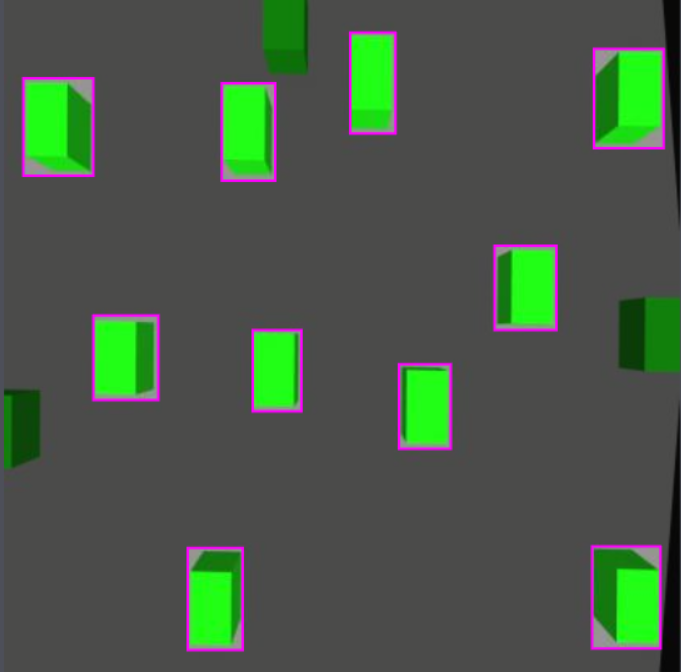
\includegraphics[width=6cm]{labeling-process-1} }
		\label{fig:labeling-process-1} }%
	\hspace{0.5cm}
	\subfloat[four targets within the frame]{
		{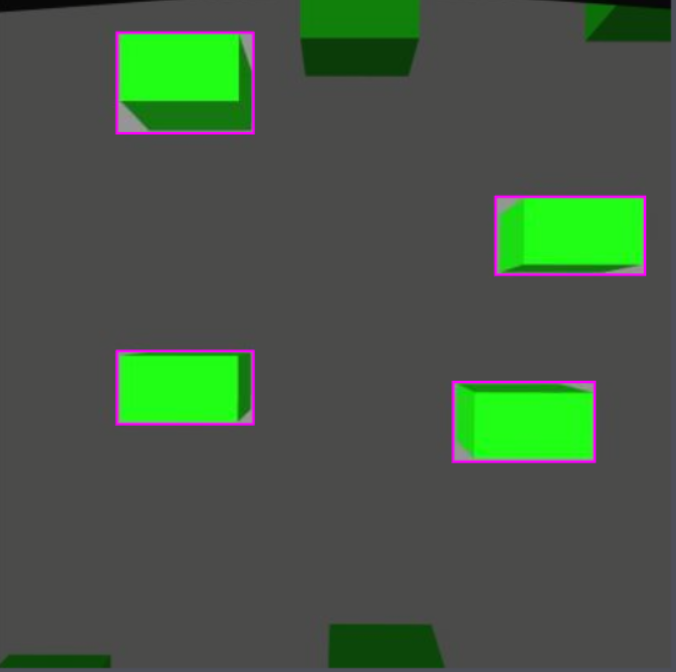
\includegraphics[width=6cm]{labeling-process-2} }
		\label{fig:labeling-process-2} }%
	\caption{%
		\protect\subref{fig:labeling-process-1} 
		Labeling 10 targets and
		\protect\subref{fig:labeling-process-2} 
		labeling 4 targets.}%
	\label{fig:labeling-targets}%
\end{figure}


For the model training, we relied on \textsc{yolo}v5 which is an open
source family of object detection models and architectures built in 
PyTorch. \textsc{yolo}v5 is based on deep learning schemes such as 
\gls{cnn} to train models given large data sets. There are different
versions of \textsc{yolo}v5, a compact version that does not
require a lot of processing power, and a full version that 
is more suitable for large data sets. We trained our model many times 
using different hardware and \textsc{gpu}s, we also tried performing 
data augmentation on our data set using built in methods in Roboflow 
which allowed us to make the data set larger and enhance the performance 
of the model. The data augmentation process resulted in creating three 
images for each image that we have, in that process, images are mixed
together and shuffled, or put in different directions with an amount of
rotation that will make the image look new once again to the model, 
thus training it better.

The tool we used to run the model training was Google 
Collaborate which allowed us to either use our personal hardware or 
make use of external resources allocated specifically for research 
purposes by Google itself. In Google Colab, we can choose the runtime 
type to either be the internal \textsc{cpu}, textsc{gpu} or an external 
resources from Google. A remote connection was made to Google's server 
and we trained one of our models using an excellent \textsc{gpu} 
allocated by google called Nvidia Tesla-K80 which is a \textsc{gpu} 
accelerator with 560 MHz core, 10 GHz effective memory clock, and 24GB 
GDDR5 vRAM.

The results we got were better than what we got using our personal 
\textsc{gpu}s, higher precision and confidence intervals were 
accomplished, but it was still not the best solution that could be made. 
Later, we started tweaking the model and changing all the possible 
variables to see how the model performs. Tweaking the model involves 
changing many things, such as the batch size, the number of epochs, the 
learning rate, the optimizer, and other small changes that resulted in 
different outcomes. 
After that, we managed to have access to Qatar University's servers, we 
contacted the \textsc{its} department to connect to one of the 
research-purpose servers and do the training on it. So in total, we had 
three different resources, personal hardware and \textsc{gpu}s, Google 
Collab's free \textsc{gpu}s, and the university servers. The results we 
got from the three different resources were different, and the 
performance was increasingly improving with the better resources and 
hardware used for model training. 

% In the next section I willshow the different images that we got from the training and compare between the different results. This step cannot be done until the training is finished using the servers.

\textbf{Model Performances }

For the first model, we used the small version of \textsc{yolo}v5 which is 
more \textsc{gpu} friendly and takes shorter training time.
We made use of data augmentation for this model, the batch size was 
sixteen to avoid overloading the \textsc{gpu}, and we ran it for a 
hundred epochs only.

\begin{figure}[H] 
	\centering
	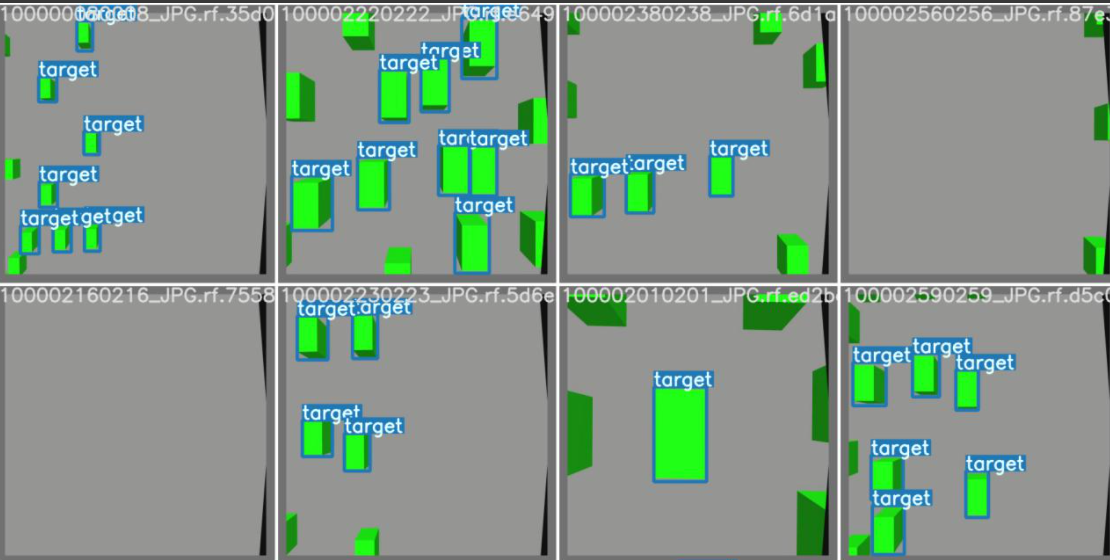
\includegraphics[width=1.0\textwidth, height=7cm]{model-1-output} 
	\caption{Model No. 1 output} \label{fig:model-1-output} 
\end{figure}

The main evaluation metrics are the precision and recall: 
\begin{figure}[H] 
	\centering
	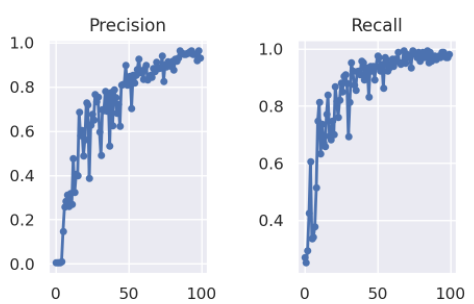
\includegraphics[width=0.8\textwidth]{model-1-performance} 
	\caption{Model No. 1 performance evaluation} \label{fig:model-1-performance} 
\end{figure}

The precision is an essential indicator of a model's performance, it shows 
how precise the predictions are. 
It is calculated by the following formula: 
\[ Precision =  \frac{True Positives}{True Positives + False Positives} \]

Another important metric is the recall value, which shows how many of the 
true positives were found and classified correctly, it is calculated by:
\[ Recall =  \frac{True Positives}{True Positives + False Negatives} \] 
From \cref{fig:model-1-performance}, we observe that both the precision and recall start low 
at the beginning, and increase as more epochs pass. By the hundredth 
epoch, both precision and recall are at a high value which is very close 
to one.  

The last metric is the mean average precision (mAP), as we can see in 
\cref{fig:model-1-mAP}, the value starts low at the beginning and 
increases with epochs passing, for the mAP 0.5 it is very high and close
to one, which means that it was a hit and a target was detected 
correctly most of the time. However, in the mAP 0.5:0.95 the final value 
is lower and barely above 0.8 which means that there are different mAP 
values over different IoV (intersection over union) thresholds ranging 
between 0.5:0.95, this is not and optimal result and it could be 
improved with better resources.


\begin{figure}[H] 
	\centering
	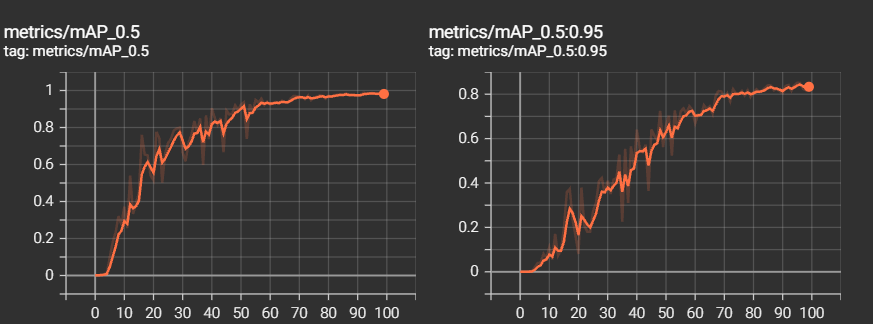
\includegraphics[width=0.8\textwidth]{model-1-mAP} 
	\caption{Model No. 1 mAP} \label{fig:model-1-mAP} 
\end{figure}
 





\subsection{Physical components}

The most critical parts in the hardware
architecture are the Raspberry Pi and the drone. 
We started by configuring the Raspberry Pi micro\textsc{sd} card,
flashed it with Ubuntu 18.04 desktop version,
and installed Parrot Olympe successfully. 
Then we plugged in the Wi-Fi dongle adapter
in a \textsc{usb}~2.0 port in the Raspberry Pi, 
and the \textsc{os} discovered it automatically. 

Now everything is ready to test the 
\anafi drone, so we have connected the
Raspberry Pi to the drone using built-in WiFi
to allow Raspberry to send/receive control and status 
instructions to the drone. 
For connecting Raspberry Pi and the laptop, 
we used the external WiFi adapter and turned 
on the hotspot feature to create an access point,
and this made the process so convenient because 
once the Raspberry Pi boots up, it turns on the 
access point, and the user can connect to it 
easily and execute scripts using \textsc{ssh} 
protocol or open the graphical interface 
control using the \textsc{vnc} feature.

We executed the takeoff and move forward scripts,
and it worked successfully, so we got the green 
light to continue. 
Regarding the power supply we were thinking 
of modifying the drone's battery by removing the 
plastic shield because of the drone's payload restrictions 
and limitations, but everything changed after testing 
the drone's maximum payload. As shown in \cref{fig:payload}
we attached \SI{190}{\gram} of Raspberry Pi and Arduino boards
to see the effect on the performance and flight and
battery drain percentage. 
The drone has taken off  successfully, 
and the flight was normal but, we faced an expected 
battery drain that went from 
\SI{100}{\percent} to \SI{90}{\percent} in 
\SI{1.5}{\minute}.
This means the drone can fly up to 
\SI{15}{\minute} which is \SI{10}{\minute} 
less than the default battery time 
which will be considered in design constraints.
In our case, the total weight of our parts is equal
to \SI{170}{\gram} which will add small time
to the battery life.

\begin{figure}[H]
	\centering
	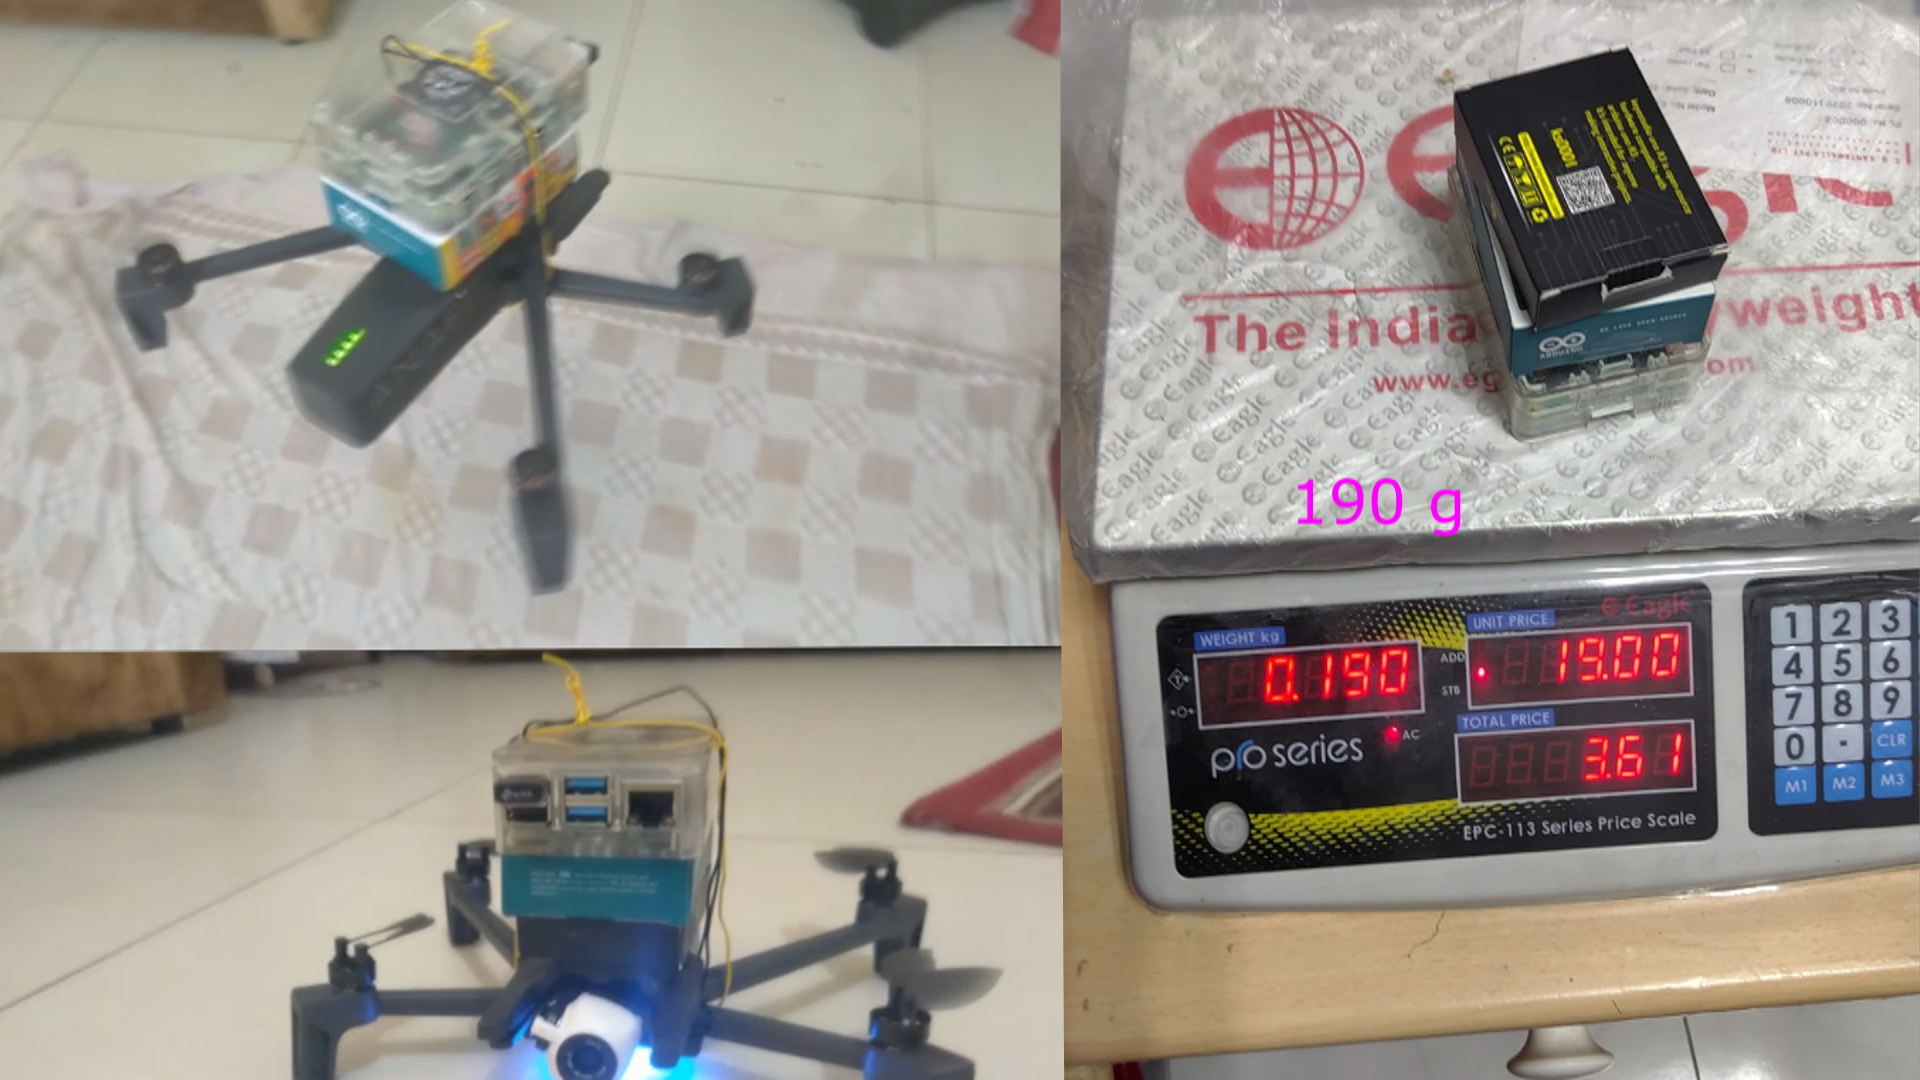
\includegraphics[width=0.6\textwidth]{payload.png}
	\caption{The drone payload}
	\label{fig:payload}
\end{figure} 


We have done another experiment regarding the response time 
of the drone after sending a command to it from the Raspberry Pi. 
Calculating the response time was by starting a timer when 
sending the command and stopping it when the 
state of the drone changes. 
The experiment was done on simulation using Sphinx,
then we have moved to the real world using the \anafi drone.
From \cref{tab:respone-time}, 
we can see that all the results are less than \SI{1}{\second}
which satisfied our response time constraint.
Another thing we can conclude from the table is that 
the response time of the real world is less than 
the simulation, and this is predictable since the simulation
depends on the \textsc{gpu} power and processing time. 

\begin{table}[tbp]
	\centering
	\caption{The response time of the drone after sending a control command.}
	\label{tab:respone-time}
	\begin{tabular}{ p{6cm} p{4cm} p{4cm} }
		\toprule
		\textit{} & \textit{Simulation} & \textit{Real-world}\\ \midrule
		Motor ramping for takeoff (seconds)  & 0.3506 & 0.0323     \\
		Move while flying (seconds) & 0.7441  & 0.1511   \\
		\bottomrule
	\end{tabular}
\end{table} 

For the Raspberry Pi power supply, we have ordered it 
online because it is not available locally and 
it arrived after 17 days at the post office.
Regarding the connection, there are 
two different options to connect as shown in \cref{fig:connection}.
For option A we can use USB-A to power the Raspberry directly without
need to solder any wires,
but there is some internal resistance.
In option B it power the Raspberry Pi through the \textsc{gpio} 
interface by soldering two wires to the power board and 
connect to pin 4 and 6 in the Raspberry Pi board,
this option has small internal resistance compared to option A.
For simplicity, we will choose option A and we will 
follow the instruction of the manufacture by choosing 

the thickest and shortest possible USB cable to reduce 
the cable loss and voltage drops~\cite{makerfocus}.

 \begin{figure}[tbp]
 	\centering
 	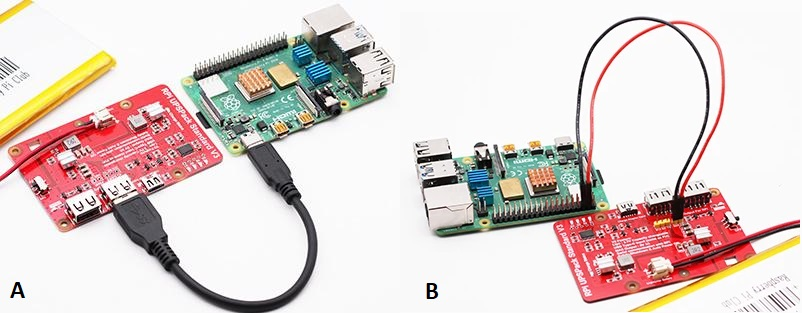
\includegraphics[width=0.5\textwidth]{connection.png}
 	\caption{The Raspberry Pi and power board connection.}
 	\label{fig:connection}
 \end{figure}   

Since all the components are available as shown 
in \cref{fig:components}, we can now assemble 
all the parts in one piece and start testing the whole system.
We have used the zip tie to hold the components and to
make sure everything sticks together. After trying to use the 
nylon straps tape to attach the components to the drone 
we have figured out that it blocks the fan 
and sensors in the bottom of the drone, 
so normal wires attached to the sides of the drone were 
used as a temporary solution. Also, we are considering 
designing a 3D printed holder to make the process more 
flexible and convenient in future advancements but for now,
we will stick to the simpler way. As shown in 
\cref{fig:full-hardware} all the parts are in one system 
and test flight was smooth and everything works perfectly. 

 \begin{figure}[tbp]
	\centering
	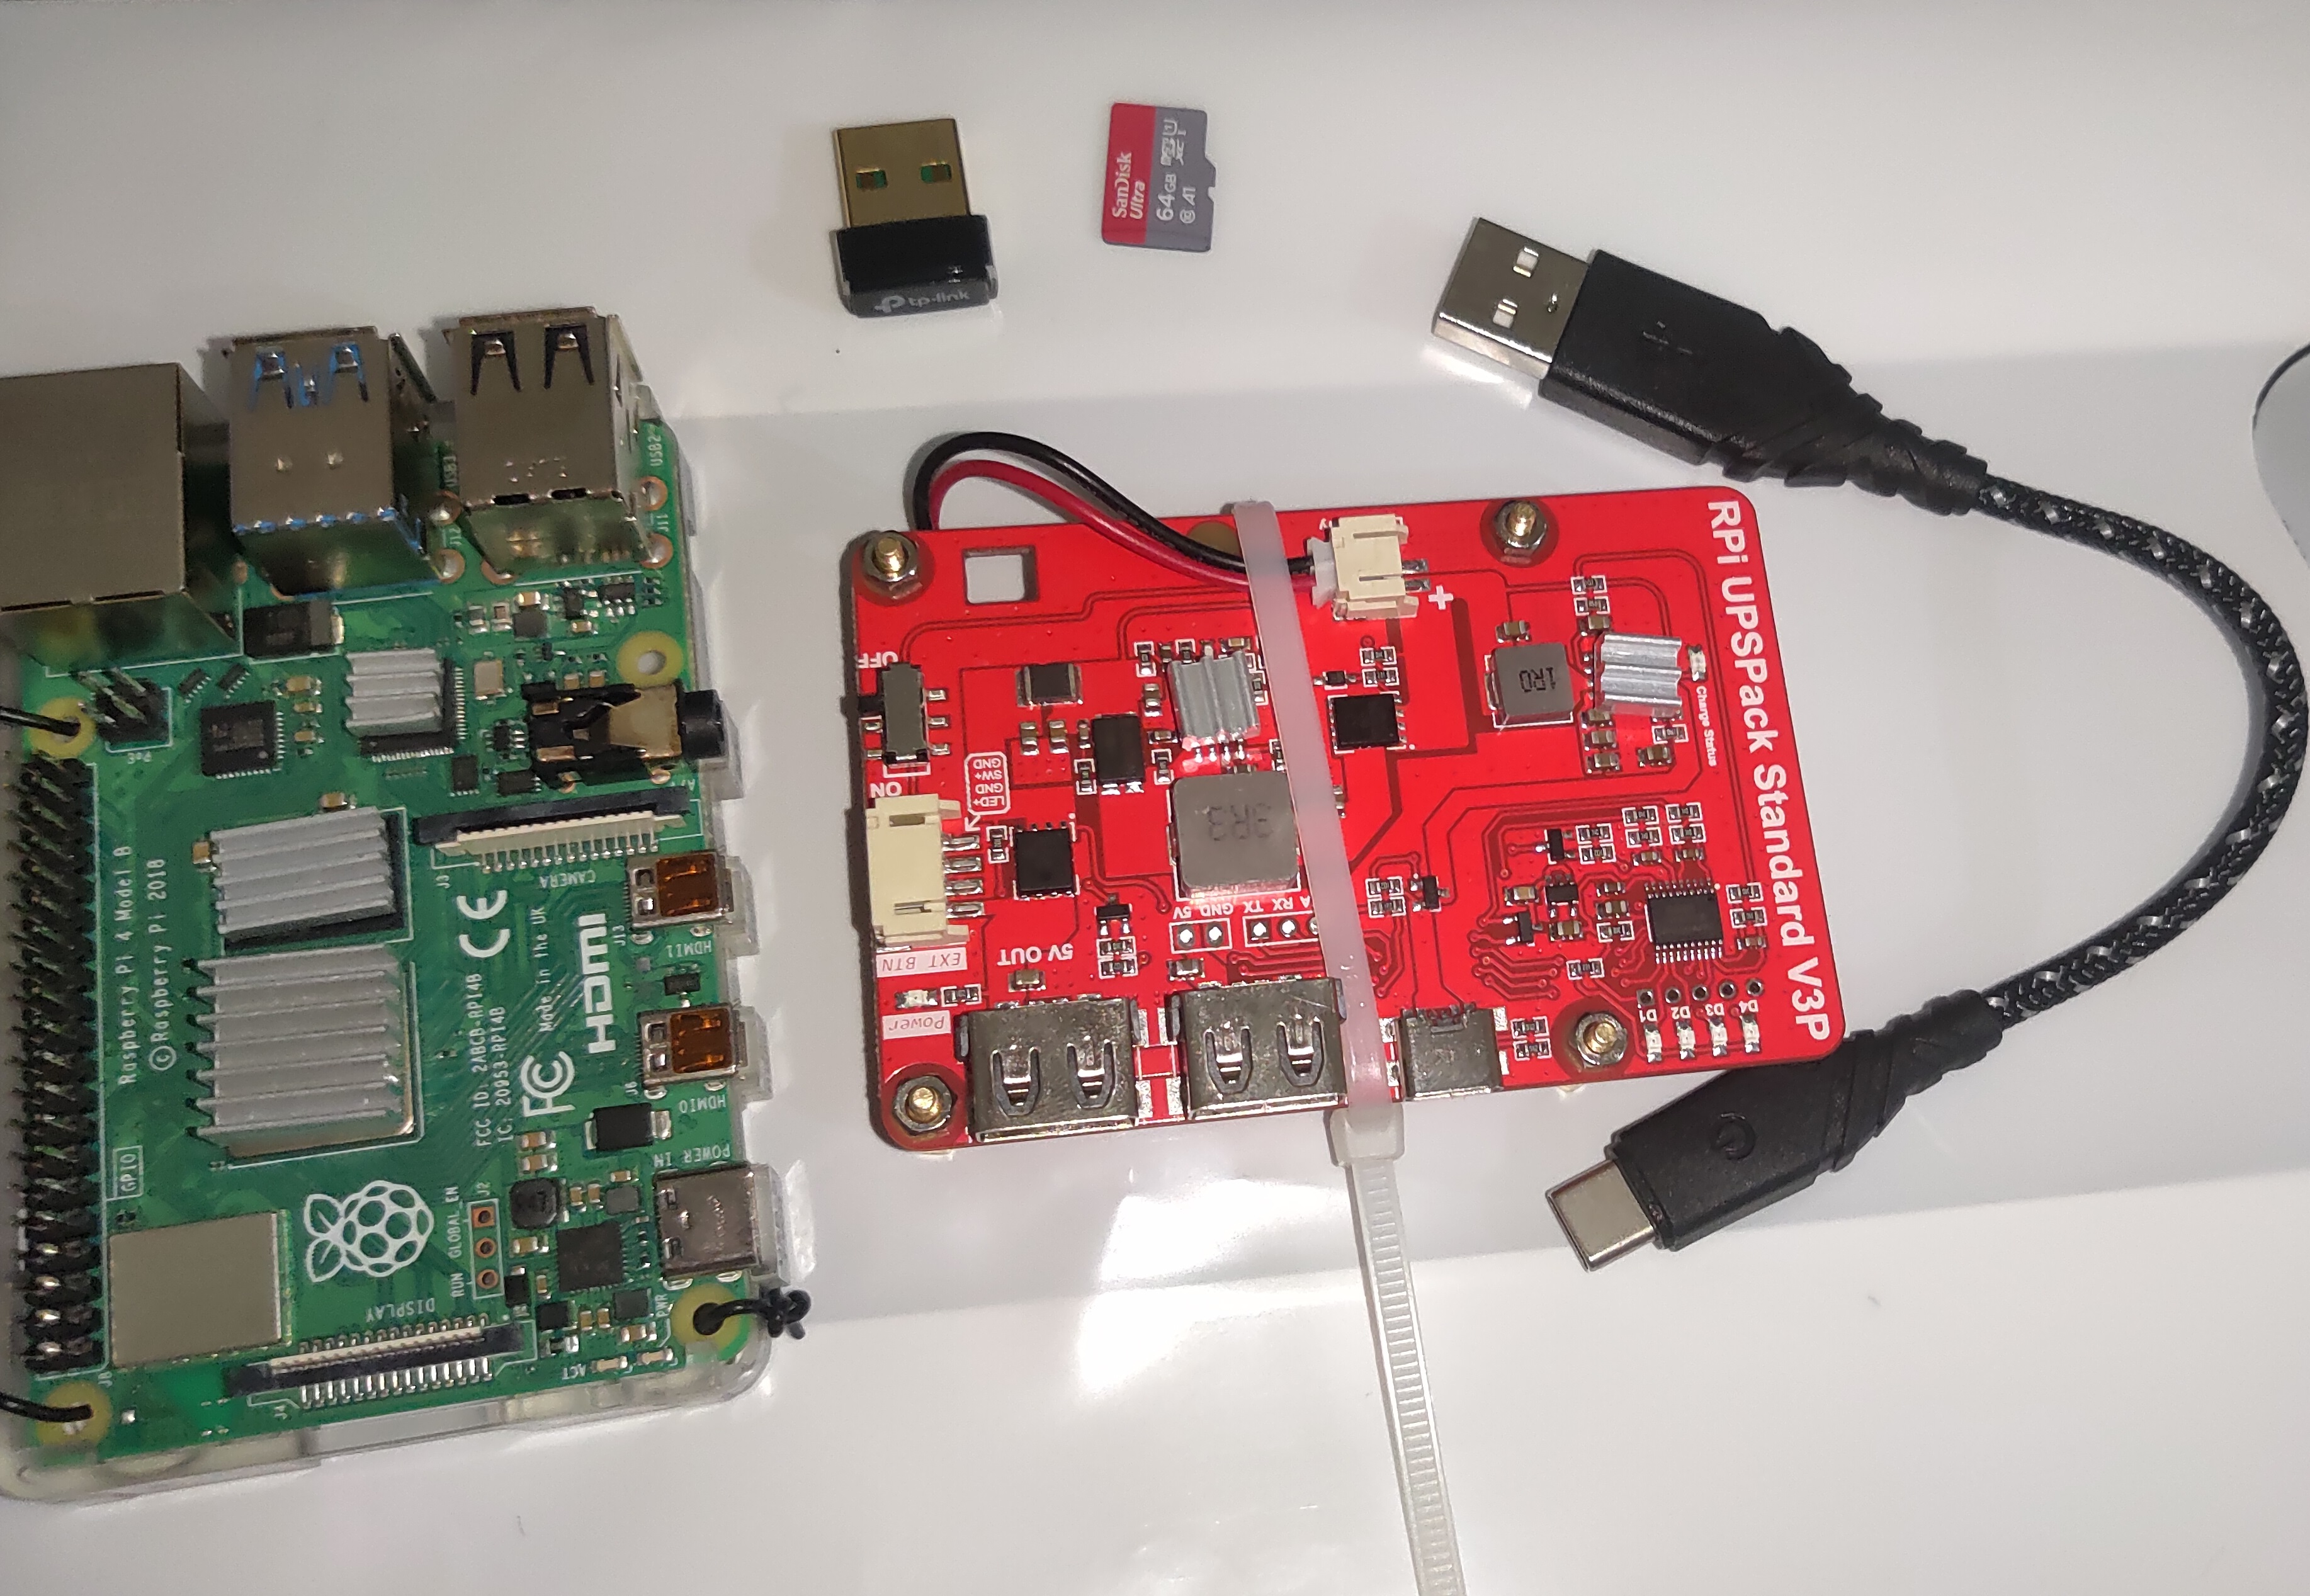
\includegraphics[width=0.5\textwidth]{components.jpg}
	\caption{All components needed.}
	\label{fig:components}
\end{figure}

  \begin{figure}[tbp]
 	\centering
 	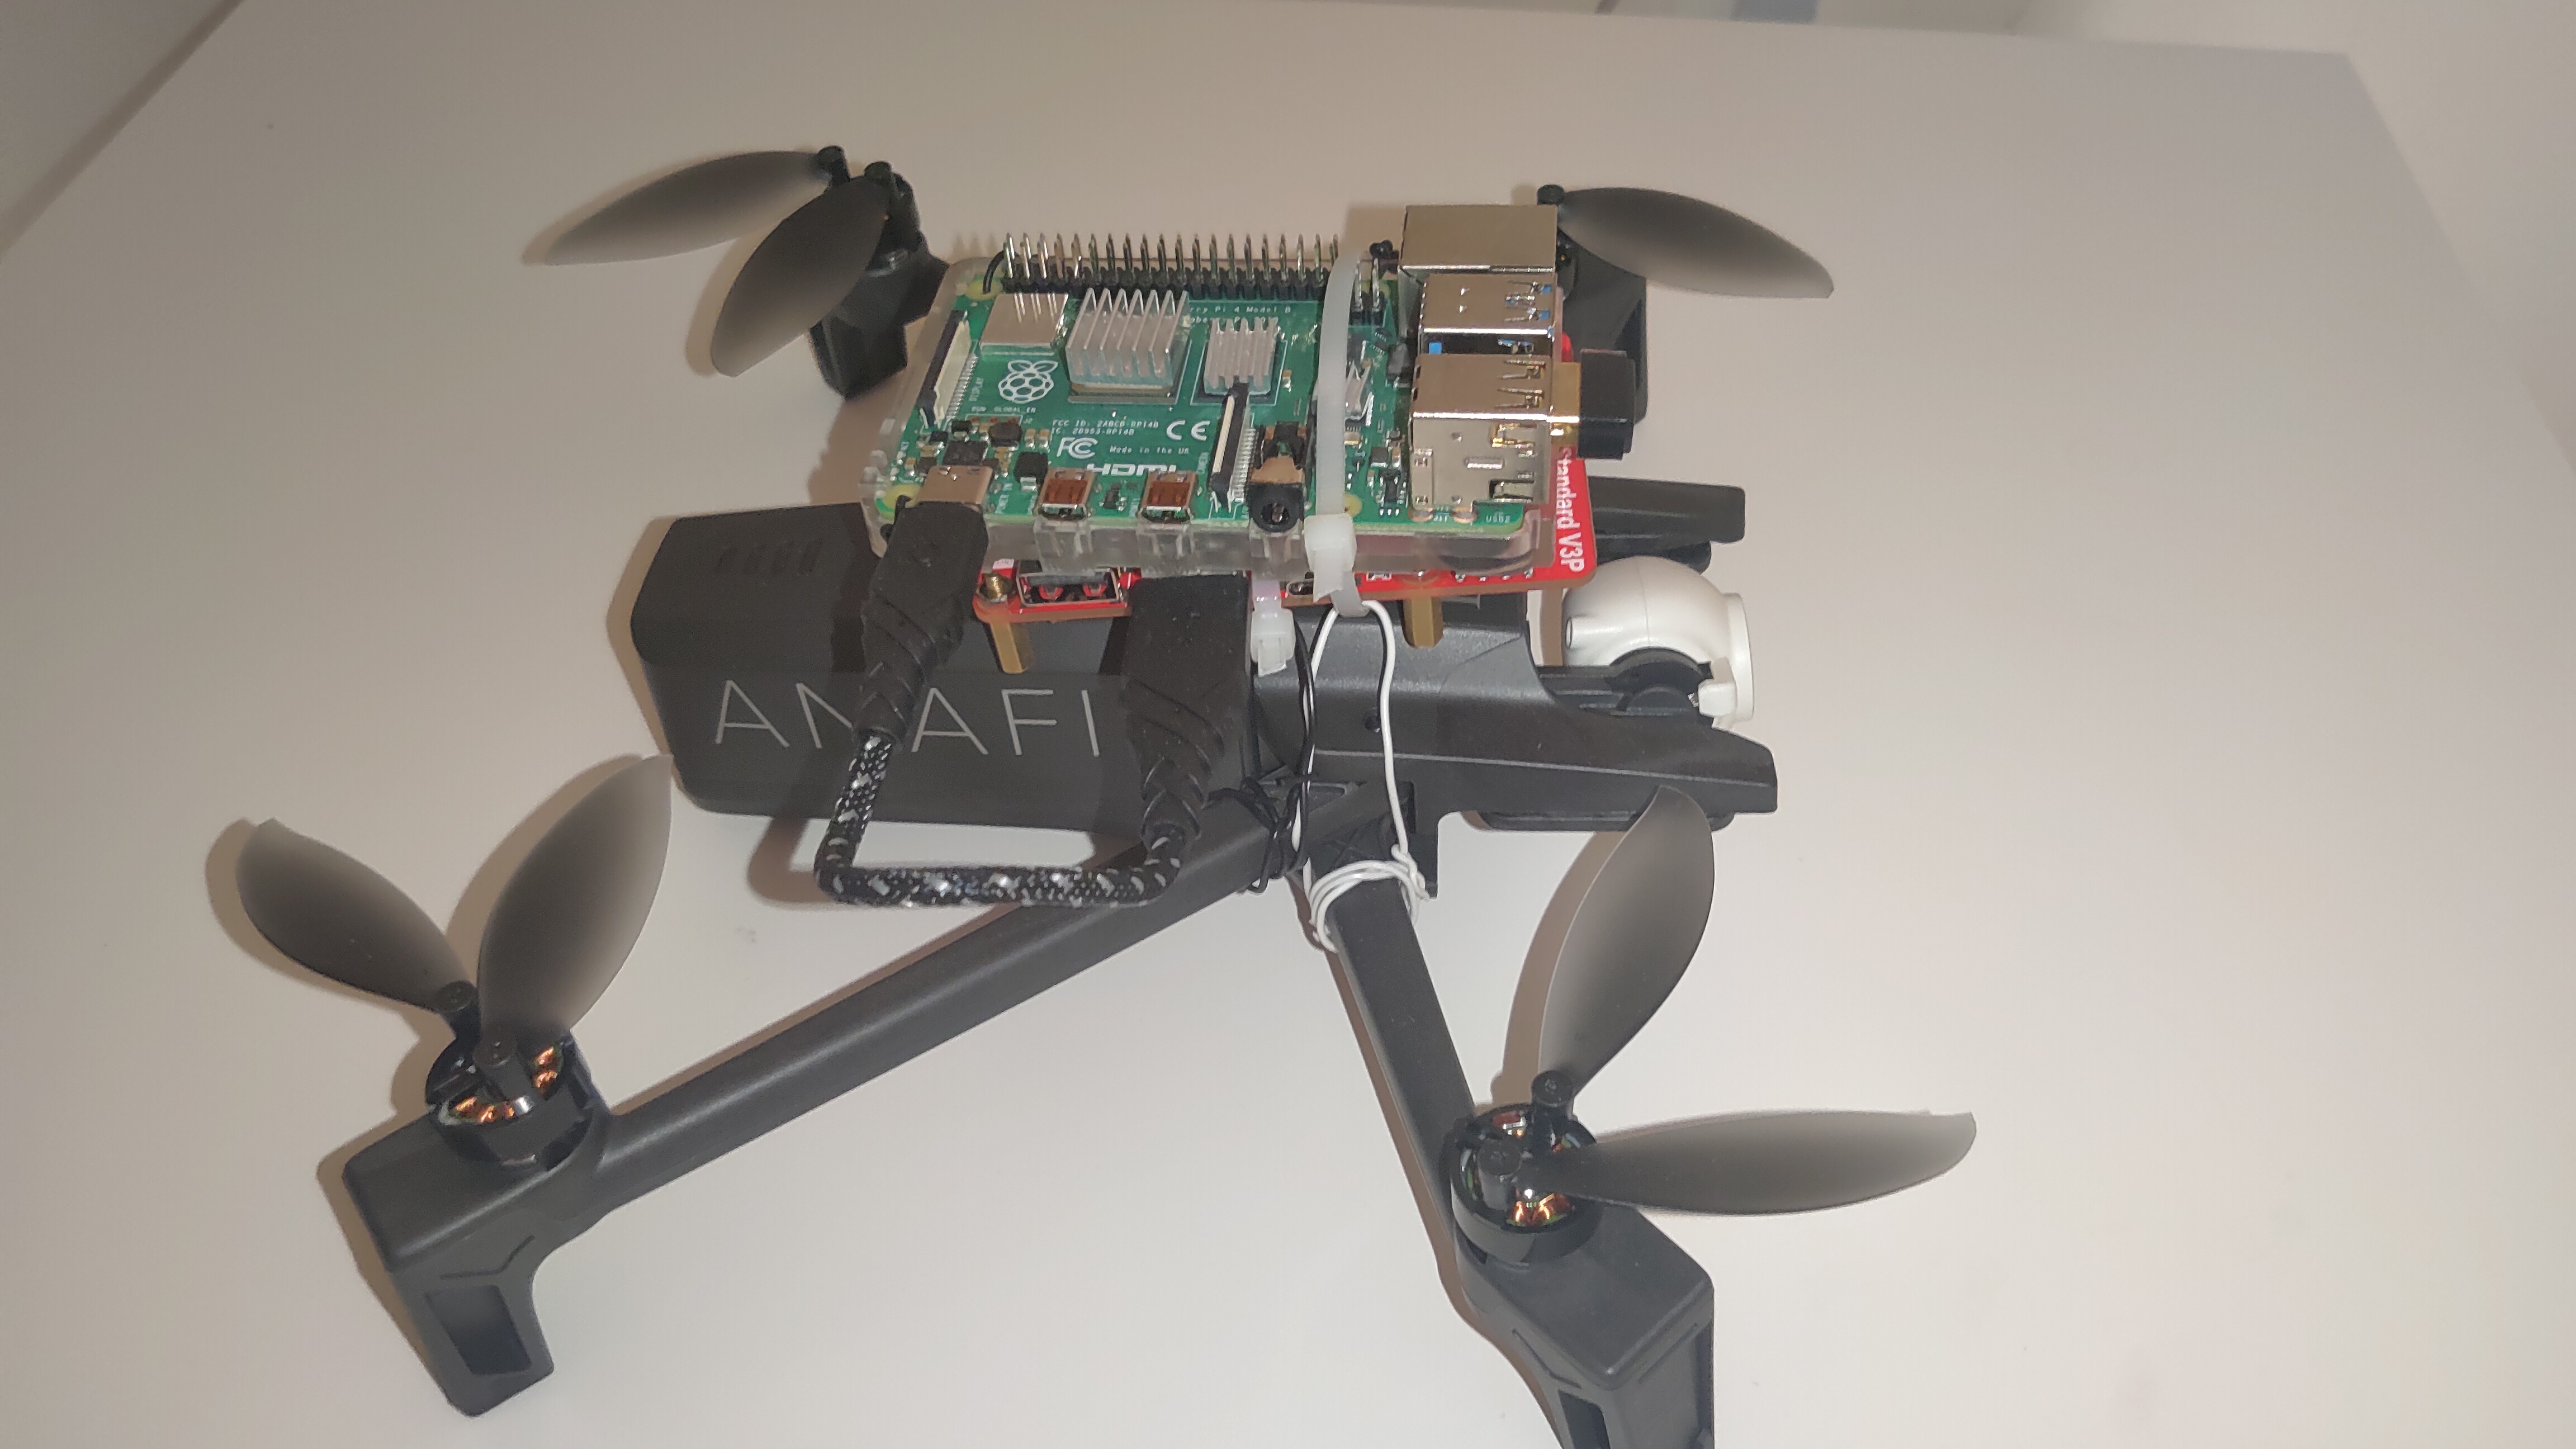
\includegraphics[width=0.5\textwidth]{full-hardware.jpg}
 	\caption{Full hardware system.}
 	\label{fig:full-hardware}
 \end{figure}  

\end{document}
